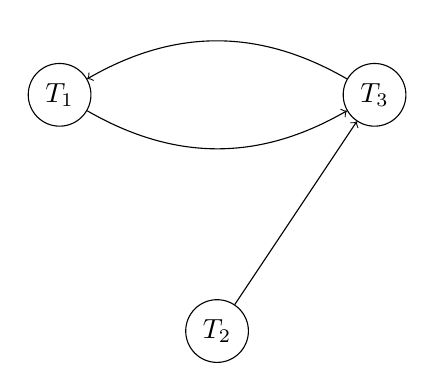
\begin{tikzpicture}
\tikzstyle{label} = [above,yshift=5pt];
\tikzstyle{res}=[minimum width=20pt,minimum height=5pt,draw];
\tikzstyle{pro}=[circle,draw];
\tikzstyle{alloc}=[->];
\node [pro] (v2) at (-2,-0.5) {$T_1$};

\node [pro] (v4) at (0,-3.5) {$T_2$};
\node [pro] (v5) at (2,-0.5) {$T_3$};


\draw [alloc,in=30,out=150] (v5) edge (v2);
\draw [alloc] (v4) edge (v5);
\draw [alloc,in=210,out=-30] (v2) edge (v5);
\end{tikzpicture}